% interactcadsample.tex
% v1.03 - April 2017

\documentclass[]{interact}

\usepackage{epstopdf}% To incorporate .eps illustrations using PDFLaTeX, etc.
\usepackage{subfigure}% Support for small, `sub' figures and tables
%\usepackage[nolists,tablesfirst]{endfloat}% To `separate' figures and tables from text if required

\usepackage{natbib}% Citation support using natbib.sty
\bibpunct[, ]{(}{)}{;}{a}{}{,}% Citation support using natbib.sty
\renewcommand\bibfont{\fontsize{10}{12}\selectfont}% Bibliography support using natbib.sty

\theoremstyle{plain}% Theorem-like structures provided by amsthm.sty
\newtheorem{theorem}{Theorem}[section]
\newtheorem{lemma}[theorem]{Lemma}
\newtheorem{corollary}[theorem]{Corollary}
\newtheorem{proposition}[theorem]{Proposition}

\theoremstyle{definition}
\newtheorem{definition}[theorem]{Definition}
\newtheorem{example}[theorem]{Example}

\theoremstyle{remark}
\newtheorem{remark}{Remark}
\newtheorem{notation}{Notation}


% tightlist command for lists without linebreak
\providecommand{\tightlist}{%
  \setlength{\itemsep}{0pt}\setlength{\parskip}{0pt}}



\usepackage{hyperref}
\usepackage[utf8]{inputenc}
\def\tightlist{}


\begin{document}


\articletype{ORIGINAL RESEARCH ARTICLE}

\title{Diagnostic biface acquisition through trade with distinct
extralocal communities of practice: A case study from the American
Southeast}


\author{\name{Robert Z. Selden, Jr.$^{a}$, Catherine G.
Cooper$^{b}$, and John E. Dockall$^{c}$}
\affil{$^{a}$Heritage Research Center, Stephen F. Austin State
University; Department of Biology, Stephen F. Austin State University;
Texas Archeological Research Laboratory, The University of Texas at
Austin; and Cultural Heritage Department, Jean Monnet
University; $^{b}$National Center for Preservation Technology and
Training, National Park Service; $^{c}$Stantec, Inc.}
}

\thanks{CONTACT Robert Z. Selden,
Jr.. Email: \href{mailto:zselden@sfasu.edu}{\nolinkurl{zselden@sfasu.edu}}, Catherine
G. Cooper. Email: , and John E. Dockall. Email: }

\maketitle

\begin{abstract}
Nodule size and mechanical flaking properties have been advanced to
account for assemblage level differences in the morphology of stone
tools within regions where raw material is abundant. However, in
instances where lithic raw materials---larger nodules in
particular---were scarce, did traders interact with brokers from
distinct extralocal communities to acquire large bifaces? Gahagan
bifaces are among those implements diagnostic of Formative/Early Caddo
material culture (CE 800 - 1250); although, due to a lack of local
production evidence, it is also widely accepted that Gahagan bifaces
were not manufactured by the Caddo. This study asks whether Caddo
traders engaged in commerce with brokers from discrete extralocal
communities of practice to acquire Gahagan bifaces. Results demonstrate
significant differences in Gahagan biface geochemistry and shape based
on color group assignment, suggesting that Gahagan biface shape was
conditioned by raw material color. Given these findings, it is posited
that Caddo traders acquired Gahagan bifaces from two distinct
communities of practice, where local raw material and production
differences resulted in Gahagan bifaces that were unique in color,
geochemistry, and shape.
\end{abstract}

\begin{keywords}
American Southeast; Caddo; NAGPRA; lithics; raw material color; pXRF;
computational archaeology; museum studies; digital humanities;
non-Western art history; STEM; STEAM
\end{keywords}

\begin{quote}
``The question of questions for mankind---the problem which underlies
all others, and is more deeply interesting than any other---is the
ascertainment of the place which man occupies in nature, and of his
relation to the universe of things.'' \textbf{--H. Thomas Henry Huxley},
\emph{Man's Place in Nature}
\end{quote}

\hypertarget{introduction}{%
\section{Introduction}\label{introduction}}

\begin{figure}
\includegraphics[width=1\linewidth]{ms_files/figure-latex/map} \caption{Location of Mounds Plantation and Gahagan Mound, illustrating the geographic extent of the Red River basin (blue) and the ancestral Caddo area (dashed white).}\label{fig:figmap}
\end{figure}

\begin{figure}
\includegraphics[width=1\linewidth]{ms_files/figure-latex/fig02} \caption{Gahagan bifaces from Caddo burial caches at Gahagan Mound and Mounds Plantation.}\label{fig:figbifaces}
\end{figure}

\hypertarget{methods-and-results}{%
\section{Methods and Results}\label{methods-and-results}}

\hypertarget{color}{%
\subsection{Color}\label{color}}

Gahagan bifaces were scanned at 600 dpi using an HP ScanJet G4050.
Images were subsequently transferred to a transparent background in
Photoshop in preparation for analysis using the \texttt{colordistance}
package in R \citep{R, RN11200}. A histogram binning method was used to
group similar colors, and pairwise distances between histograms were
computed using earth mover's distance, yielding two distinct raw
material color groups \citep{RN11201, RN11200}.

\begin{figure}
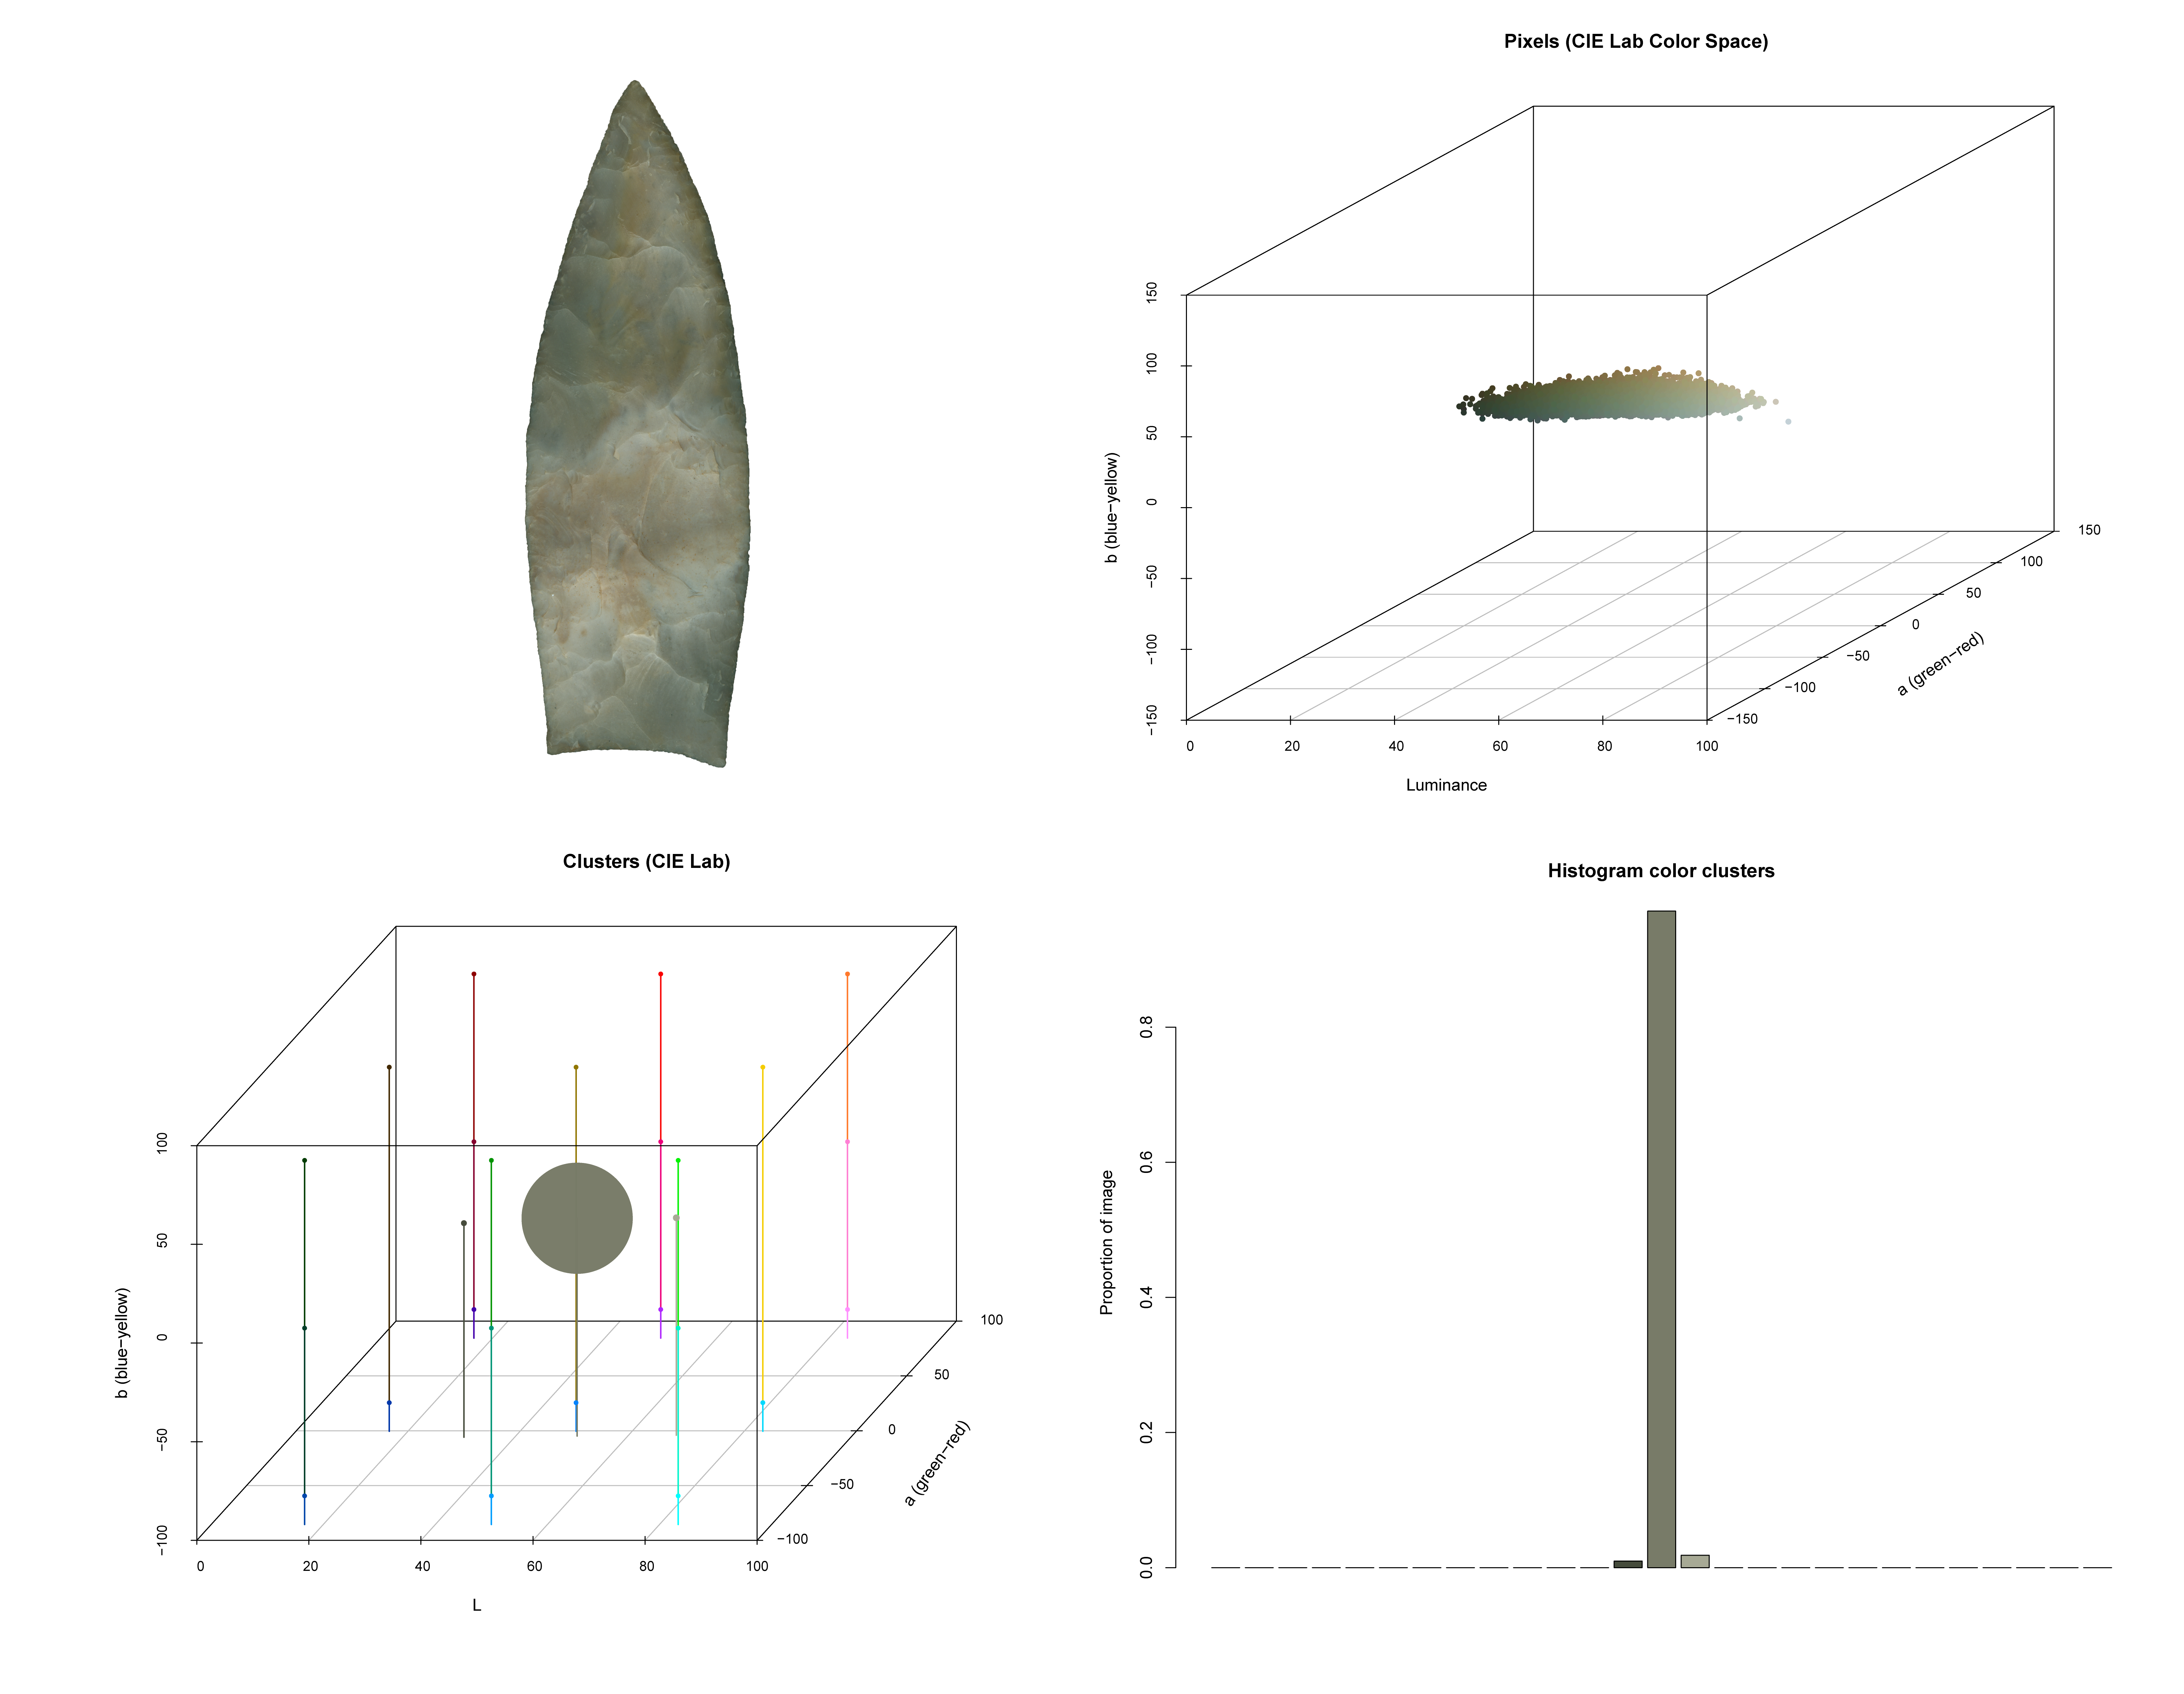
\includegraphics[width=1\linewidth]{ms_files/figure-latex/fig3} \caption{Color binning process for a single object; adapted from Weller and Westneat (2019:Figure 2). In a, image of a Gahagan biface with a transparent background; b, 3D scatterplot of 10,000 non-background pixels in RGB color space; c, clusters from histogram displayed in RGB color space; and d, histogram showing the proportion of non-background pixels assigned to each bin.}\label{fig:colorout}
\end{figure}

Bifaces were coded as ColorGroup A and ColorGroup B using the output
from a neighbor-joining tree, calculated using the color distance
matrix. To test whether bifaces differ in color according to ColorGroup
assignment, the color distance matrix was exported and joined with the
categorical data. Those data were used in a permutational multivariate
analysis of variance in the \texttt{vegan} package to evaluate whether
biface color differs by raw material color group \citep{R, vegan}, where
the two raw material color groups were found to differ significantly
(\emph{permutations = 10,000; \textbf{Pr(\textgreater F) = 9.999e-05}}).

\begin{figure}
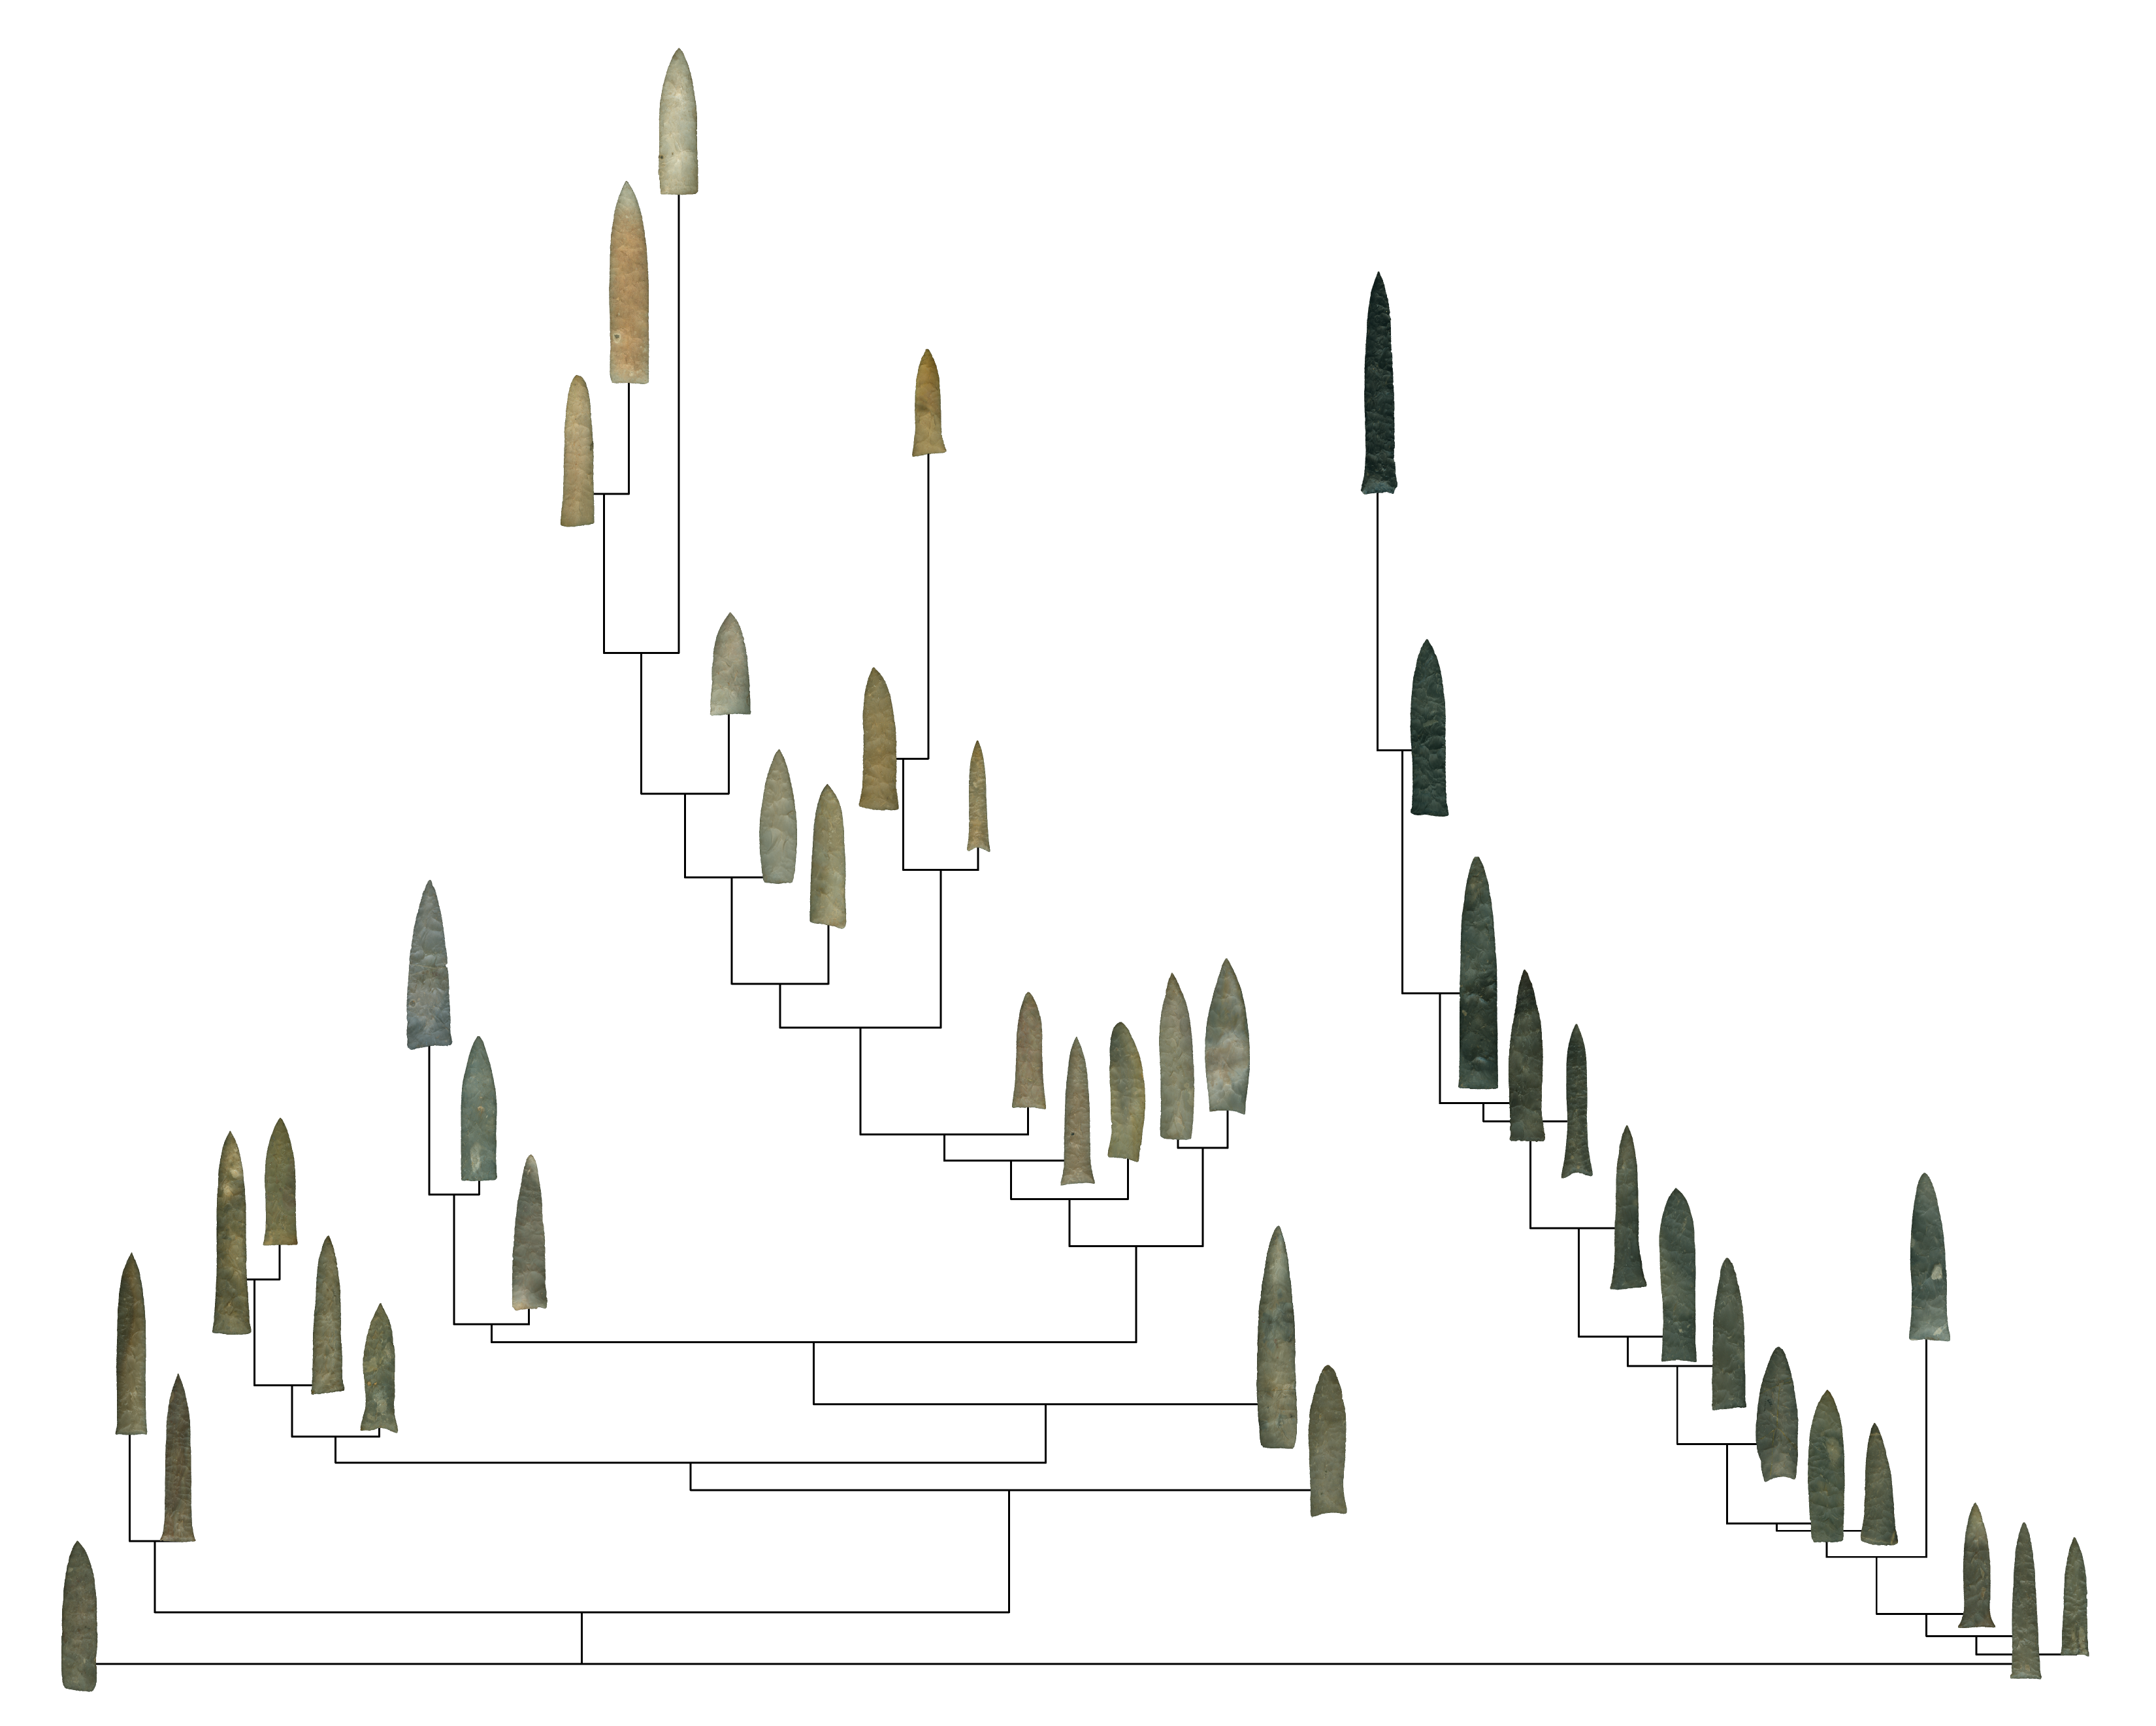
\includegraphics[width=1\linewidth]{ms_files/figure-latex/fig4} \caption{Neighbor-joining tree illustrating color data for the two Gahagan biface ColorGroups; ColorGroup B (left) and ColorGroup A (right).}\label{fig:colorspace}
\end{figure}

\hypertarget{geochemistry}{%
\subsection{Geochemistry}\label{geochemistry}}

A Bruker Trace Vi handheld portable X-ray Fluorescence (pXRF) instrument
was used to collect elemental data. The instrument was transported to
the Williamson Museum and Louisiana State Exhibit Museum and set up in a
nose-down configuration, where samples were raised into contact with the
pXRF window using a pair of small jacks cushioned with fabric. Due to
surface irregularities, the contact between the window and the bifaces
was imperfect, resulting in variable count and response rates during
data collection.

Data was collected using the following scan parameters: 40kV, 35uA, Ti
25um:Al 300um filter for 180 seconds. Peaks in each spectrum were
identified manually in Bruker's Artax software; once elements were
identified, the spectrum was evaluated by the Artax Bayesian statistical
program to separate overlapping peaks. The Artax results were exported
as net peak areas normalized to the silicon (Si) peak.

Elemental data were subsequently imported to R for a principal
components analysis (PCA), followed by a permutational multivariate
analysis of variance (perMANOVA), used to assess whether raw material
differs between sites \citep{R, vegan}.

\begin{figure}
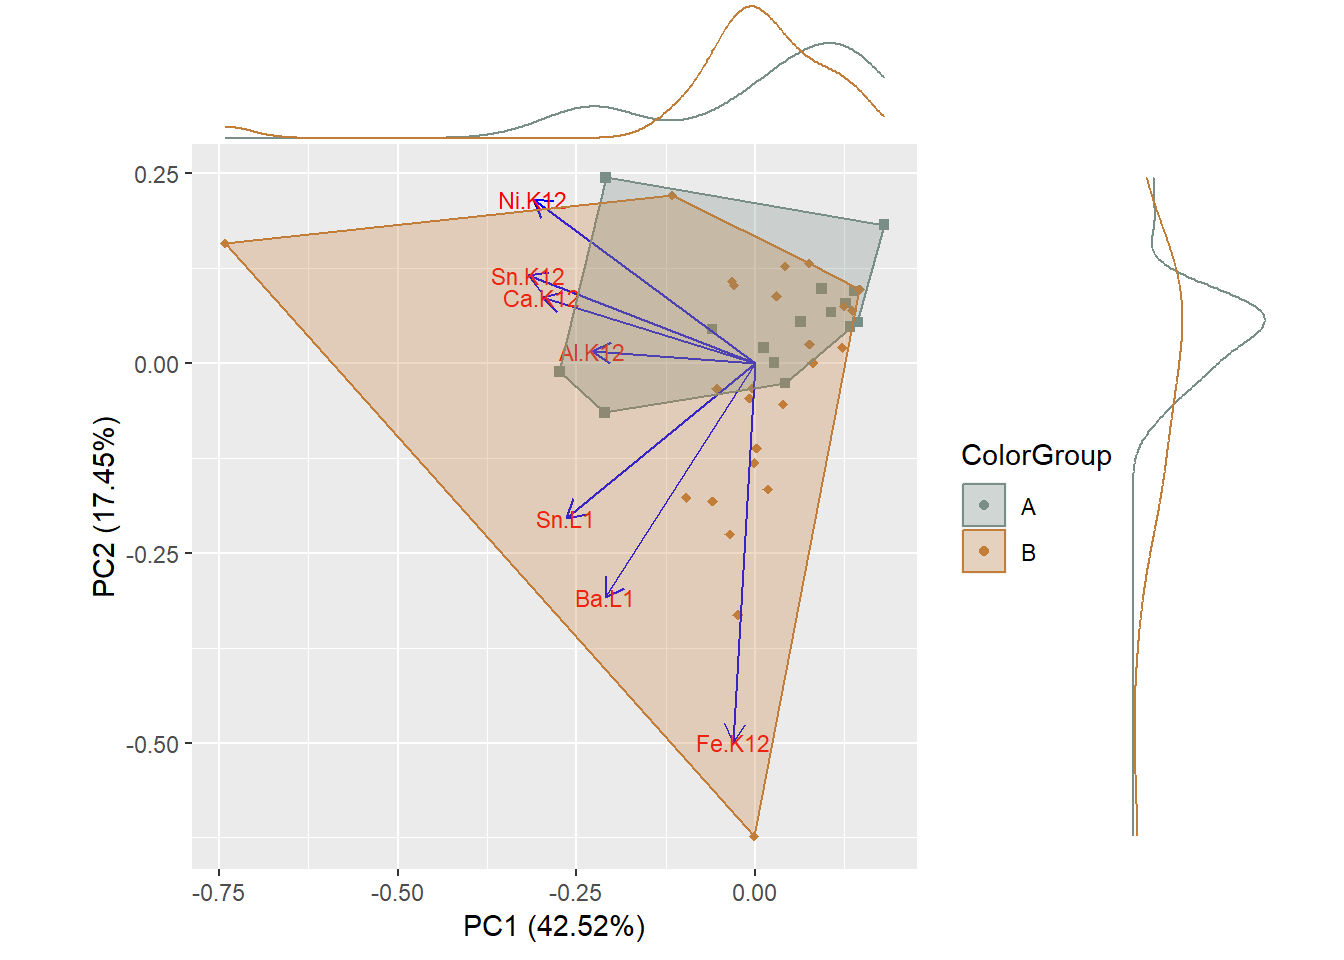
\includegraphics[width=1\linewidth]{ms_files/figure-latex/pcaelem-1} \caption{Composite image illustrating the plot of first two principal components by site using a correlation matrix, illustrating 59.32 percent of cumulative shape variation, where gray squares denote Color Group A, and orange triangles denote Color Group B.}\label{fig:figsite}
\end{figure}

The PCA illustrates 59.97 percent of the variation in the sample among
PC1 (42.52 percent) and PC2 (17.45 percent). The perMANOVA demonstrated
that elemental values differ significantly by raw material color groups
(\emph{permutations = 10,000; \textbf{Pr(\textgreater F) = 0.0406}}).

\hypertarget{geometric-morphometrics}{%
\subsection{Geometric morphometrics}\label{geometric-morphometrics}}

Landmark data were aligned to a global coordinate system
\citep{RN8477, RN7502, RN11622, RN11623, RN11563}, achieved through
generalized Procrustes superimposition \citep{RN11138, RN478, RN1646} in
R using the \texttt{geomorph} and \texttt{RRPP} packages
\citep{RN1655, RN11775, RN11530, RN1774, RN9565}. Procrustes
superimposition translates and rotates the coordinate data to allow for
comparisons among objects, while also scaling each biface using
unit-centroid size---the square root of the sum of squared distances
from each landmark to the specimen's centroid
\citep{RN11139, RN11140, RN11564, RN478}. The \texttt{geomorph} package
uses a partial Procrustes superimposition that projects the aligned
specimens into tangent space subsequent to alignment in preparation for
the use of multivariate methods that assume linear space
\citep{RN11141, RN11142, RN1646, RN11563}.

Principal components analysis \citep{RN1746} was used to visualize shape
variation among the elliptical bifaces, and the scatterplot represents
the dispersion of shapes in tangent space
\citep{RN8633, RN5616, RN11143, RN7550}. Shape ranges described by each
principal axis are commonly visualized using thin-plate spline warping
of a reference image \citep{RN1731, RN479}.

\begin{figure}
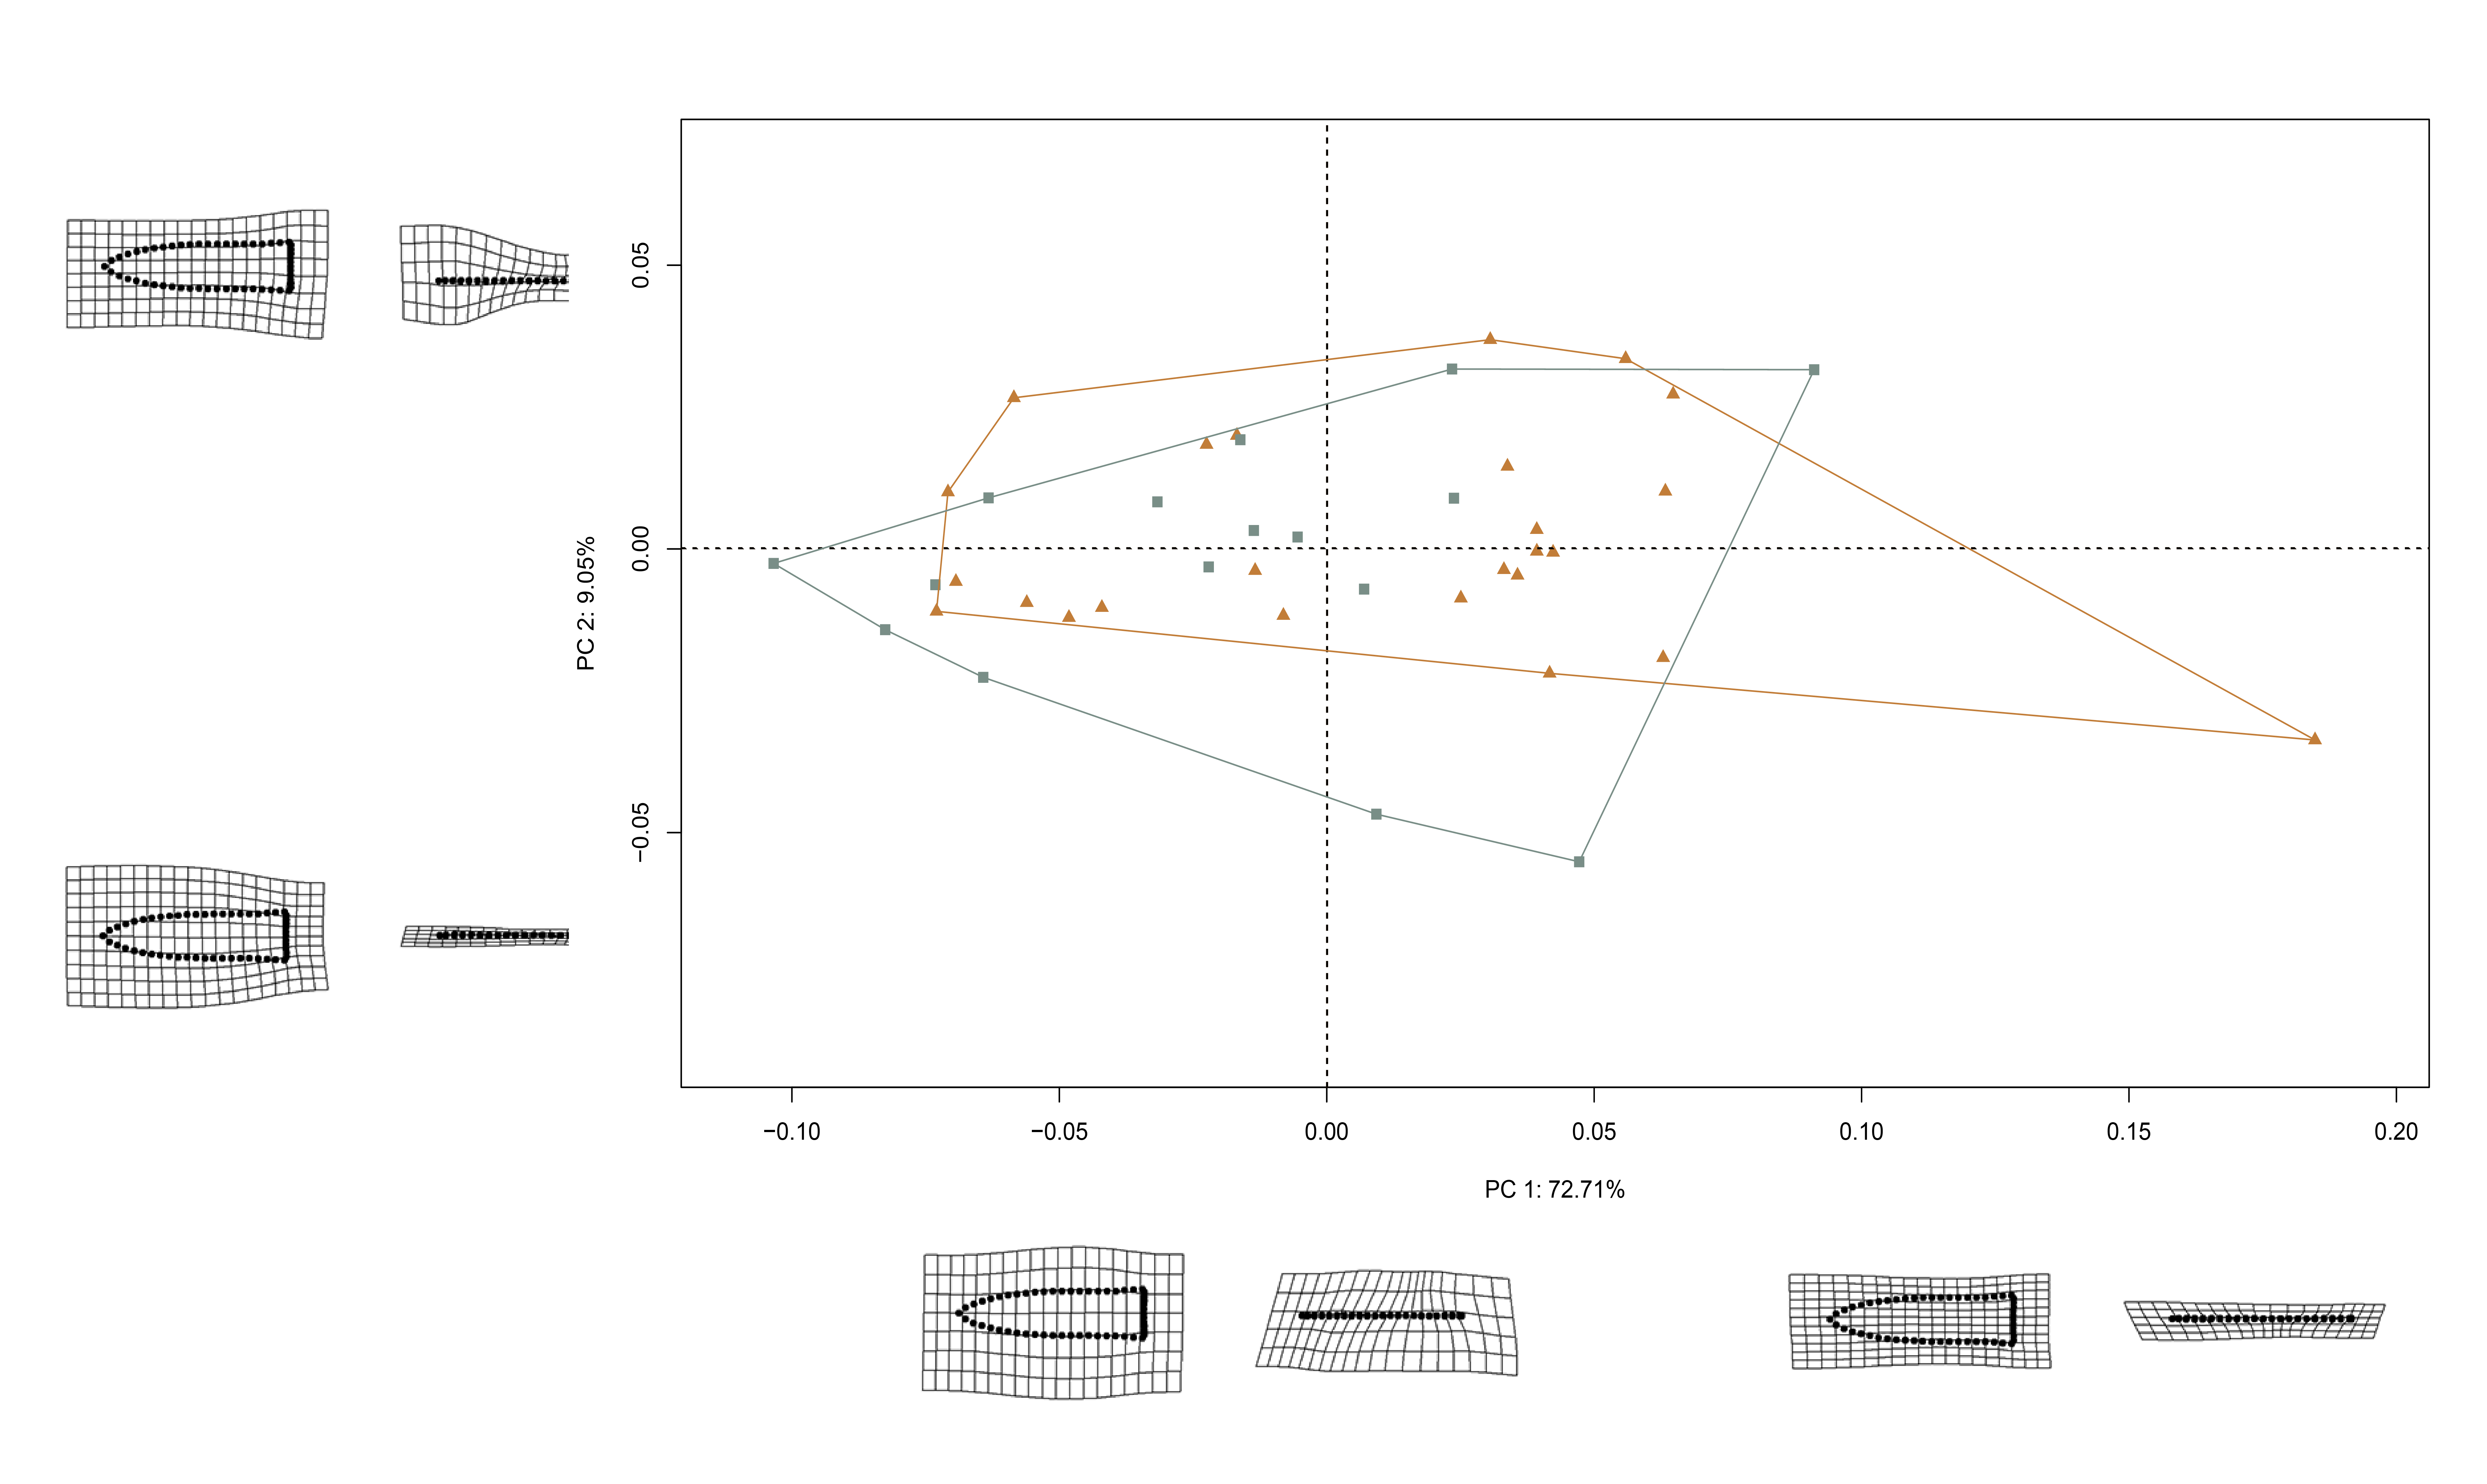
\includegraphics[width=1\linewidth]{ms_files/figure-latex/pcashape-1} \caption{PCA summarizing shape variation in Gahagan bifaces from Color Group A (gray squares) and Color Group B (orange triangles).}\label{fig:figpcashape}
\end{figure}

To assess whether \texttt{shape} and \texttt{size} differs by
\texttt{ColorGroup}, Procrustes ANOVAs \citep{RN1749} were run that
enlist effect-sizes (zscores) computed as standard deviates of the
generated sampling distributions \citep{RN1756}. A residual
randomization permutation procedure (RRPP; n = 10,000 permutations) was
used for all Procrustes ANOVAs \citep{RN1655, RN11775}, which has higher
statistical power and a greater ability to identify patterns in the data
should they be present \citep{RN1719}.

\hypertarget{discussion-and-conclusion}{%
\section{Discussion and Conclusion}\label{discussion-and-conclusion}}

\hypertarget{acknowledgements}{%
\section*{Acknowledgement(s)}\label{acknowledgements}}
\addcontentsline{toc}{section}{Acknowledgement(s)}

We extend our gratitude to the Caddo Nation of Oklahoma, the Caddo
Nation Tribal Council, Tribal Chairman, and Tribal Historic Preservation
Office for their continued guidance and support of our work, as well as
access to NAGPRA and previously repatriated collections. Thanks also to
the Williamson Museum and the Louisiana State Exhibit Museum for
providing access to the Gahagan bifaces, and to Bruce Kayser for his
time and guidance with pXRF questions. RZS also extends his gratitude to
Emma Sherratt, Kersten Bergstrom, Lauren Butaric, Dean C. Adams, and
Michael L. Collyer for their constructive criticisms and suggestions
throughout the development of this research program.

\hypertarget{disclosure-statement}{%
\section*{Disclosure statement}\label{disclosure-statement}}
\addcontentsline{toc}{section}{Disclosure statement}

The authors declare no conflicts of interest.

\hypertarget{data-management}{%
\section*{Data management}\label{data-management}}
\addcontentsline{toc}{section}{Data management}

All data and analysis code associated with this project are openly
available through the
\href{https://github.com/seldenlab/gahaganmorph.5}{GitHub} repository,
which is digitally curated on the Open Science Framework
(\href{https://osf.io/3jb94/}{DOI 10.17605/OSF.IO/3JB94}). Additionally,
images of all Gahagan bifaces used in this study are openly available to
view/download through an open access comparative collection
(\url{https://scholarworks.sfasu.edu/ita-gahaganbiface/}). The
supplementary materials include all analysis data and code used in the
study, providing a means for others to reproduce (exactly) those results
discussed and expounded upon in this article. The replicable nature of
this undertaking provides others with the means to critically assess and
evaluate the various analytical components of this study
\citep{RN20915, RN20916, RN20917}, which is a necessary requirement for
the production of reliable knowledge.

Reproducibility projects in \href{https://osf.io/ezcuj/}{psychology} and
\href{https://www.cos.io/rpcb}{cancer biology} are impacting current
research practices across all domains. Examples of reproducible research
are becoming more abundant in archaeology
\citep{RN20804, RN21009, RN21001, RN9364, RN11097}, and the next
generation of archaeologists are learning those tools and methods needed
to reproduce and/or replicate research results \citep{RN21007}.
Reproducible and replicable research work flows are often employed at
the highest levels of humanities-based inquiries to mitigate concern or
doubt regarding proper execution, and is of particular import should the
results have---explicitly or implicitly---a major impact on scientific
progress \citep{RN21008}.

\hypertarget{funding}{%
\section*{Funding}\label{funding}}
\addcontentsline{toc}{section}{Funding}

Components of the analytical workflow were developed and funded by a
Preservation Technology and Training grant (P14AP00138) to RZS from the
National Center for Preservation Technology and Training, as well as
grants to RZS from the Caddo Nation of Oklahoma, National Forests and
Grasslands in Texas (15-PA-11081300-033) and the United States Forest
Service (20-PA-11081300-074). Additional funding and logistical support
was provided by the Heritage Research Center at Stephen F. Austin State
University and the National Center for Preservation Technology and
Training.

\bibliographystyle{tfcad}
\bibliography{article.bib}





\end{document}
